\documentclass[10pt]{beamer}
\usetheme{metropolis}
% all imports
\usepackage[utf8]{inputenc}
\usepackage[T1]{fontenc}
\usepackage{lmodern}
\usepackage{amsmath}
\usepackage{hyperref}
\usepackage{booktabs}
\usepackage{bm}
\usepackage[scale=2]{ccicons}
\usepackage[outputdir=build]{minted}
\usepackage{pgfplots}
\usepackage{array,colortbl,xcolor}
\usepgfplotslibrary{dateplot}
\usepackage{setspace}
\usepackage{etoolbox}
\usepackage{xspace}
\usepackage{tikz}
\usetikzlibrary{shapes,arrows,positioning,fit,backgrounds}
\usepackage{tkz-euclide}

\AtBeginEnvironment{quote}{\singlespacing}

\AtBeginEnvironment{quote}{\singlespacing}

% new commands
\newcommand{\vect}[1]{\bm{#1}}
\newcommand{\myprime}[1]{{#1}^{\prime}}
\newcommand{\grad}[2]{\nabla_{#1} {#2}}
\newcommand{\dotp}[2]{{#1}^{\top}{#2}}
\newcommand{\dotpPright}[2]{{#1}^{\top}\left({#2}\right)}
\newcommand{\outerp}[2]{\left({#1}\right){#2}^{\top}}
\newcommand{\Jacobian}[2]{\frac{\partial #1}{\partial #2}}
\newcommand{\Vocab}{\mathbb{V}}
 \DeclareMathOperator*{\argmin}{arg\,min}
 \DeclareMathOperator{\E}{\mathbb{E}}

% definitions
\definecolor{blue}{RGB}{159, 192, 176}
\definecolor{green}{RGB}{160, 227, 127}
\definecolor{orange}{RGB}{243, 188, 125}
\definecolor{red}{RGB}{253, 123, 84}
\definecolor{nephritis}{RGB}{39, 174, 96}
\definecolor{emerald}{RGB}{46, 204, 113}
\definecolor{turquoise}{RGB}{39, 174, 96}
\definecolor{green-sea}{RGB}{22, 160, 133}
\definecolor{purple}{RGB}{181, 124, 215}
% Tikzstyles for Computation Graphs

% nodes
\tikzstyle{noop} = [circle, draw=none, fill=red, minimum size = 10pt]
\tikzstyle{op} = [circle, draw=red, line width=1.5pt, fill=red!70, text=black, text centered, font=\bf \normalsize, minimum size = 25pt]
\tikzstyle{op2} = [circle, draw=orange, line width=1.5pt, fill=orange!70, text=black, text centered, font=\bf \normalsize, minimum size = 25pt]
\tikzstyle{op3} = [circle, draw=orange, line width=1.5pt, fill=orange!70, text=black, text centered, font=\bf \scriptsize, minimum size = 7pt]
\tikzstyle{placeholder} = [circle, draw=red, line width=1.5pt, fill=red!30, text=black, text centered, font=\bf  \normalsize, minimum size = 25pt]
\tikzstyle{state} = [circle, draw=blue, line width=1.5pt, fill=blue!70, text=black, text centered, font=\bf \normalsize, minimum size = 25pt]
\tikzstyle{gradient} = [circle, draw=nephritis, line width=1.5pt, fill=nephritis!60, text=black, text centered, font=\bf \normalsize, minimum size = 25pt]
\tikzstyle{gradient2} = [circle, draw=green2, line width=1.5pt, fill=green2!60, text=black, text centered, font=\bf \normalsize, minimum size = 25pt]
\tikzstyle{textonly} = [draw=none, fill=none, text centered, font=\bf \normalsize]

% edges
% \tikzstyle{tedge}  = [draw, thick, >=stealth, ->]
\tikzstyle{tedge}  = [draw, thick, >=latex, ->]
\tikzstyle{tedge_dashed}  = [draw, thick, >=latex, ->, dashed]

% namedscope
\tikzstyle{namedscope} = [circle, draw=orange, line width=1.5pt, fill=orange!60, align=center, inner sep=0pt]

% \tikzstyle{container} = [draw=none, rectangle, dotted, inner ysep=1.5em]
% \tikzstyle{novertex} = [draw=none, fill=none, text centered]
% \tikzstyle{predicate} = [ellipse, draw, thick, text centered, rounded corners, minimum size=30pt]
% \tikzstyle{aux} = [rectangle, draw, thick, text centered, rounded corners, minimum size=30pt]
% \tikzstyle{ledge}  = [draw, dashed, thick, >=stealth, ->]
% \tikzstyle{pedge}  = [draw, thick, >=stealth, ->]


\title{Adding semantic robustness\\ to dialog agents}
\date{\today}

\vspace{1.1 cm}


\author{
  Felipe Salvatore\\
  \url{https://felipessalvatore.github.io/}
  \vspace{1.1 cm}}

\institute{\textbf{IME-USP}: Instituto de Matemática e Estatística - Universidade de São Paulo}


\begin{document}


\maketitle


\begin{frame}{Sistemas de diálogo}
 criar um programa capaz de dialogar com ser humano
\begin{center}
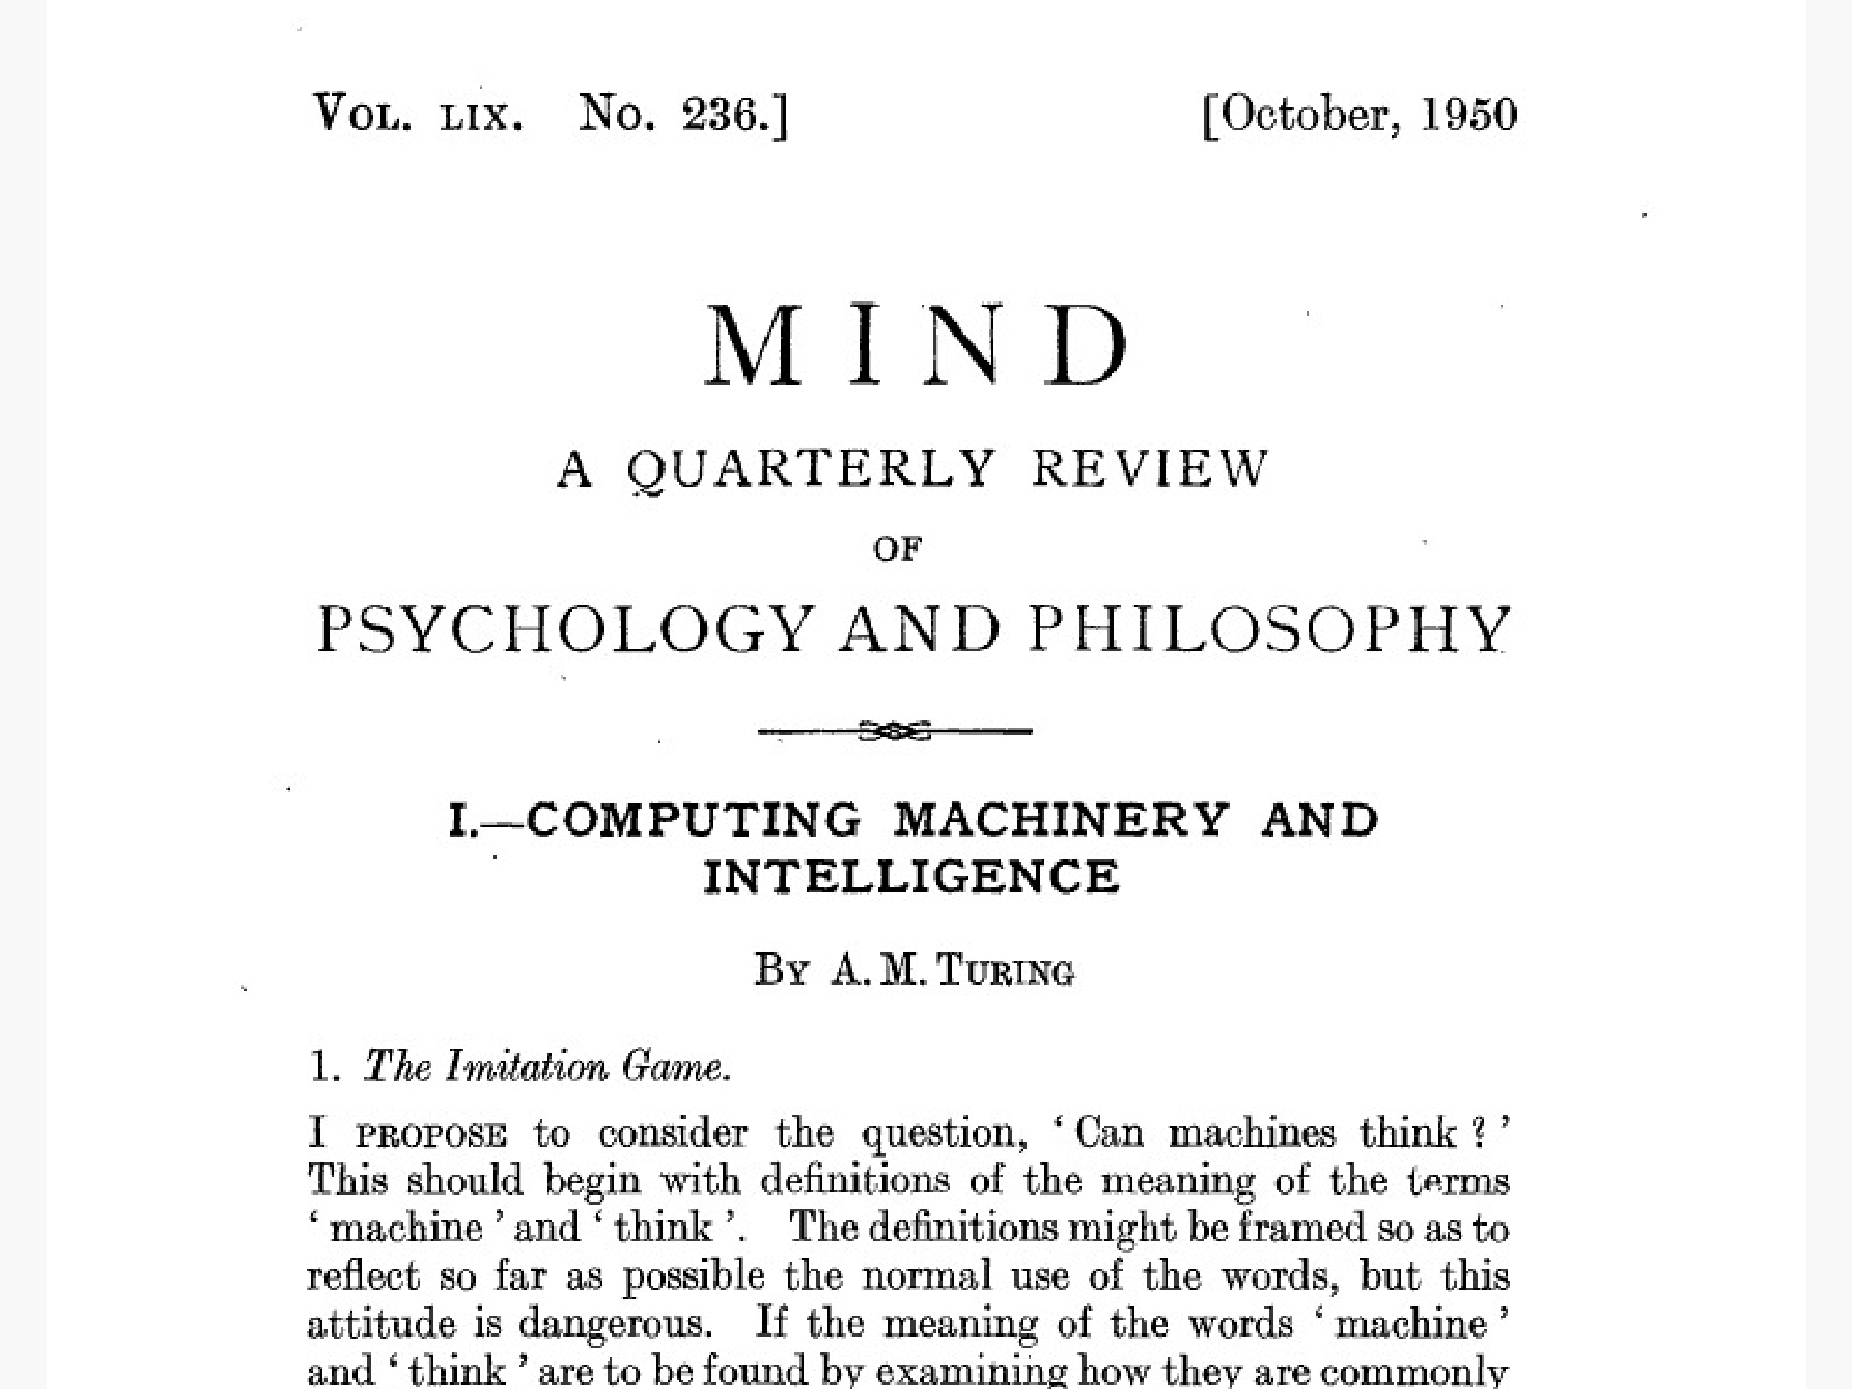
\includegraphics[scale=0.16]{images/turing.jpg}
\end{center}
\end{frame}


\begin{frame}{Sistemas de diálogo}
goal -driven vs non-goal driven
\end{frame}

\section{Sistemas de diálogo baseados em redes neurais}

\begin{frame}{Modelos de linguagem baseados em redes neurais}
Nos chamamos de \alert{modelo de linguagem} uma distribuição de probabildiade sobre uma sequencia de tokens em uma lingua natural.

\[
P(x_1,x_2,x_3,x_4) = p
\]

Em vez de usar uma abordagem que seja específica para o domínio da linguagem natural, podemos usar um modelo para predição de dados sequencias:  \textbf{uma rede recorrente (RNN)}. \\

Nossa tarefa de aprendizado é estimar a distribuição de probabilidade

\[
P(x_{n} = \text{palavra}_{j^{*}} | x_{1}, \dots ,x_{n-1})
\]

para qualquer $(n-1)$ sequencia de palavras $x_{1}, \dots ,x_{n-1}$.

\end{frame}

\begin{frame}{O modelo de linguagem com RNN}
% RNN STATE CELL ====================================
\newcommand{\rnnSimpleU}[4]{

% operations
\node[state, minimum size=40pt,#4] (h#3) {$\vect{h}^{#1}$};
\node[op, minimum size=40pt, above=30pt of h#3] (yhat#3){$\hat{\vect{y}}^{#1}$};
\node[op, minimum size=40pt,below=30pt of h#3] (e#3) {$\vect{e}^{#1}$};
\node[textonly, below=0.1pt of e#3] {{\Large#2}};

% edges
\path[tedge] (e#3) edge node[below right= -4pt] {$\vect{U}$} (h#3);
\path[tedge] (h#3) edge node[below right = -4pt] {$\vect{V}$} (yhat#3);
}

\begin{figure}[ht!]
\hspace*{-1.0cm}
\scalebox{0.8}{
\begin{tikzpicture}[auto]

% timestep 1
\rnnSimpleU{(1)}{Yes}{t1}{}

% % timestep 0
\node[state, minimum size=40pt,left=50pt of ht1] (ht0) {$\vect{h}^{(0)}$};

% % timestep 2
\rnnSimpleU{(2)}{here}{t2}{right=50pt of ht1};


% % timestep 2
\rnnSimpleU{(3)}{we}{t3}{right=50pt of ht2};


% % state transfers
\path[tedge] (ht0) edge node[above right = 2pt] {$\vect{W}$} (ht1);
\path[tedge] (ht1) edge node[above right = 2pt] {$\vect{W}$} (ht2);
\path[tedge] (ht2) edge node[above right = 2pt] {$\vect{W}$} (ht3);

% % text
\node[textonly, above=40pt of yhatt2] (result) {{\Large $P(x^{(4)}| \text{Yes, here, we})$}};

% Arrow to result
\draw[->, line width=1mm] [bend right, out=-50, distance=25pt](yhatt3.north) to  (result.east);


\end{tikzpicture}
}%\scalebox
\end{figure}


\end{frame}



\begin{frame}{GRU: Gated Recurrent Units}
\begin{center}
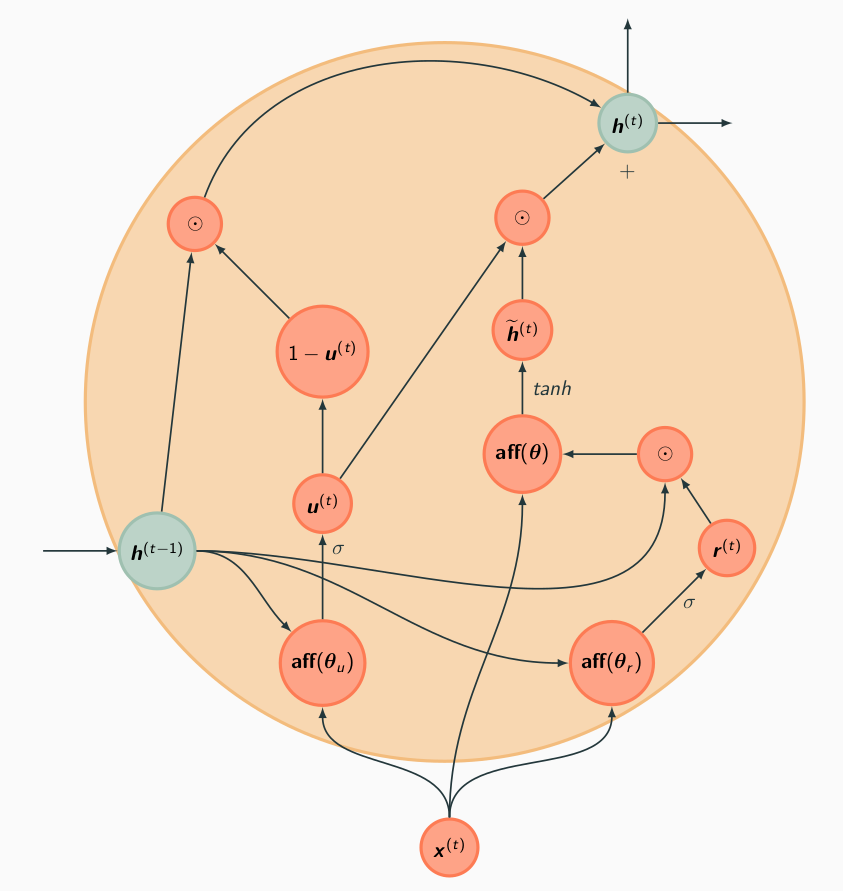
\includegraphics[scale=0.25]{images/gru.png}
\end{center}
\end{frame}


% \begin{frame}{LSTM: Long Short Term Memory}
% \begin{center}
% 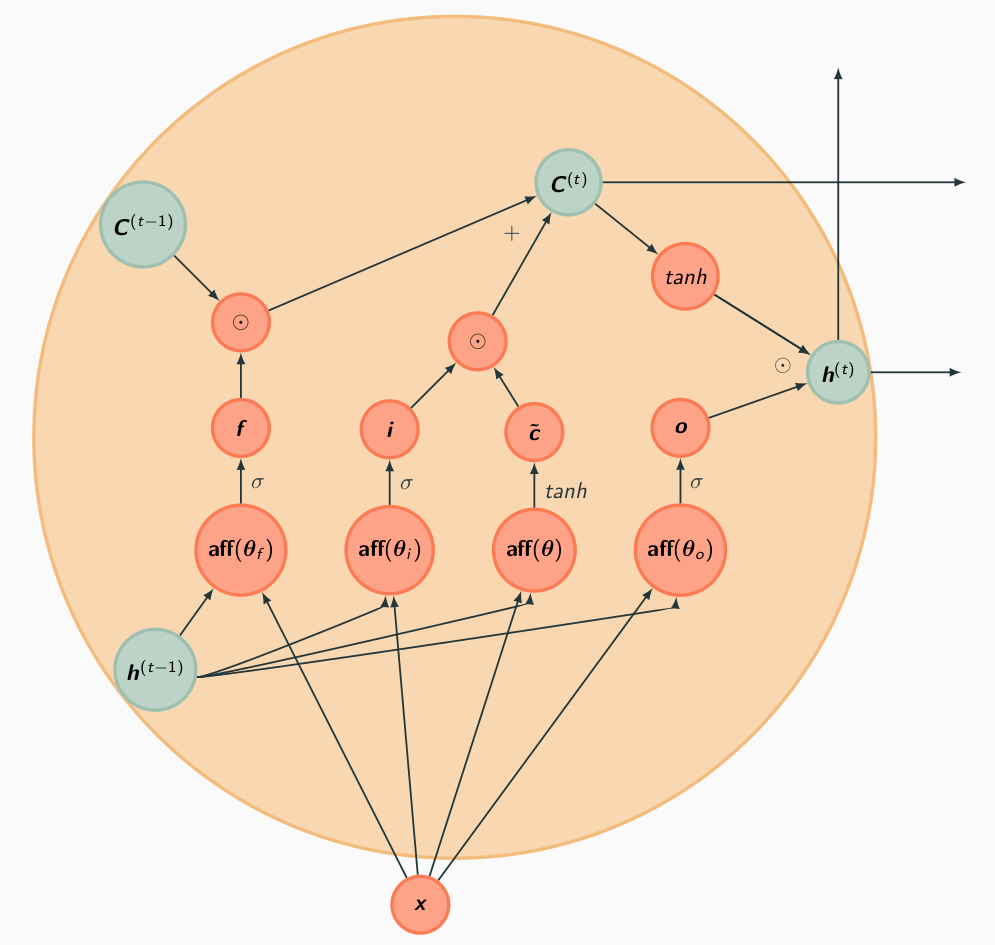
\includegraphics[scale=0.23]{images/lstm.png}
% \end{center}
% \end{frame}


\begin{frame}{Exemplo: TrumpBot\\\url{https://github.com/felipessalvatore/MyTwitterBot}}
\begin{center}
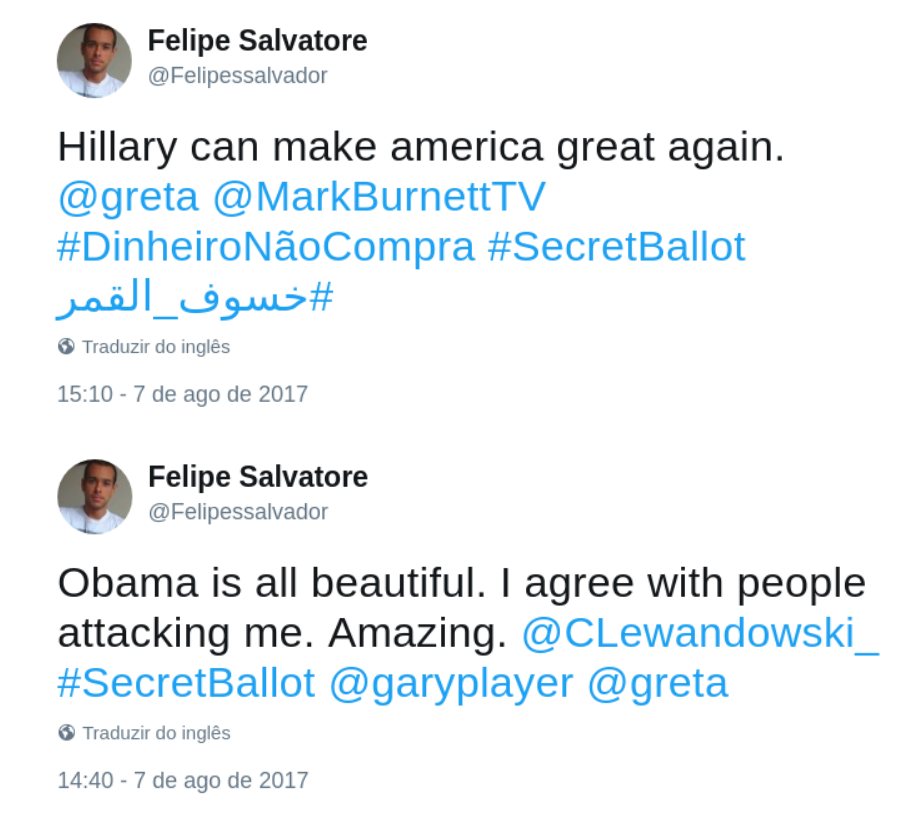
\includegraphics[scale=0.24]{images/TrumpBot.png}
\end{center}
\end{frame}


\begin{frame}{Exemplo: Funk Generator\\ \url{https://github.com/lucasmoura/funk_generator}}
\begin{quote}
\centering
É o dj que tá tocando e não sabe de nada\\ 
Eu já tô no clima e já tô no meu nome \\
Cordão de ouro no pescoço eu tô na moda \\
Com a camisa da \\
Louis \\
Vuitton \\
Pulo da morena que elas gosta\\ 
E se eu te pego no baile \\
De captiva de citroen ou de hayabusa\\ 
Tu viu a 1100 cilindradas \\
Se eu tô no litoral de cordão de ouro\\ 
De cordão de ouro no pescoço\\
\end{quote}
\end{frame}

\begin{frame}{Seq2seq: diálogo \cite{DBLP:journals/corr/VinyalsL15}}
% RNN encoder ====================================
\newcommand{\rnnencoder}[4]{

% operations
\node[state, minimum size=40pt,#4] (h#3) {$\vect{h}^{#1}$};
\node[op, minimum size=40pt,below=30pt of h#3] (e#3) {$\vect{e}^{#1}$};
\node[textonly, below=0.1pt of e#3] {{\Large#2}};

% edges
\path[tedge] (e#3) edge node[below right= -4pt] {} (h#3);
}

% RNN decoder ====================================
\newcommand{\rnndecoder}[4]{

% operations
\node[state, minimum size=40pt,#4] (h#3) {${\vect{h}^{\prime}}^{#1}$};
\node[output, minimum size=40pt, above=30pt of h#3] (yhat#3){$\hat{\vect{y}}^{#1}$};
\node[op, minimum size=40pt,below=30pt of h#3] (x#3) {$\vect{x}^{#1}$};
\node[textonly, below=0.1pt of x#3] {{\Large#2}};

% edges
\path[tedge] (x#3) edge node[below right= -4pt] {} (h#3);
\path[tedge] (h#3) edge node[below right = -4pt] {} (yhat#3);
}


\newcommand{\rnndecoderSimpl}[4]{

% operations
\node[state, minimum size=40pt,#4] (h#3) {${\vect{h}^{\prime}}^{#1}$};
\node[op, minimum size=40pt,below=30pt of h#3] (x#3) {$\vect{x}^{#1}$};
\node[textonly, below=0.1pt of x#3] {{\Large#2}};

% edges
\path[tedge] (x#3) edge node[below right= -4pt] {} (h#3);
}


\begin{figure}[ht!]
\hspace*{-1.0cm}
\scalebox{0.5}{
\begin{tikzpicture}[auto]

% timestep encoder 1
\rnnencoder{(1)}{What}{t1}{}

% timestep encoder 0
\node[state, minimum size=40pt,left=40pt of ht1] (ht0) {$\vect{h}^{(0)}$};

%  timestep encoder 2
\rnnencoder{(2)}{are}{t2}{right=40pt of ht1};

%  timestep encoder 3
\rnnencoder{(3)}{you}{t3}{right=40pt of ht2};

%  timestep encoder 4
\rnnencoder{(4)}{doing}{t4}{right=40pt of ht3};

%  timestep encoder 5
\rnnencoder{(5)}{right}{t5}{right=40pt of ht4};

%  timestep encoder 6
\rnnencoder{(6)}{now}{t6}{right=40pt of ht5};

%  timestep encoder 7
\rnnencoder{(7)}{?}{t7}{right=40pt of ht6};

% % state transfers encoder
\path[tedge] (ht0) -- (ht1);
\path[tedge] (ht1) --  (ht2);
\path[tedge] (ht2) -- (ht3);
\path[tedge] (ht3) -- (ht4);
\path[tedge] (ht4) --  (ht5);
\path[tedge] (ht5) -- (ht6);
\path[tedge] (ht6) -- (ht7);

%  timestep decoder 1
\rnndecoderSimpl{(1)}{I}{tt1}{above=190pt of ht3};

%  timestep decoder 2
\rnndecoderSimpl{(2)}{just}{tt2}{right=40pt of htt1};

%  timestep decoder 3
\rnndecoderSimpl{(3)}{start}{tt3}{right=40pt of htt2};

%  timestep decoder 4
\rnndecoder{(4)}{cleaning}{tt4}{right=40pt of htt3};


% % state transfers encoder
\path[tedge] (htt1) --  (htt2);
\path[tedge] (htt2) -- (htt3);
\path[tedge] (htt3) -- (htt4);


% text
\node[textonly, left=40pt of yhattt4] (result) {{\Large $P(x^{(5)}| \text{I, just, start, cleaning,  }\vect{h}^{(7)})$}};

% Arrow to result
\draw[->, line width=1mm] (yhattt4) to  (result.east);

% encoder to decoder
\node[state, minimum size=40pt, above=70pt of ht1] (2ht7) {$\vect{h}^{(7)}$};


% bent Arrow
\path[tedge] (ht7) edge [out=120, in=-20] node {} (2ht7);
\path[tedge] (2ht7) edge [out=90, in=180] node {} (htt1);




\end{tikzpicture}
}%\scalebox
\end{figure}


\end{frame}


\begin{frame}{Seq2seq: tradução \cite{luzfinger2017}}
% RNN encoder ====================================
\newcommand{\rnnencoder}[4]{

% operations
\node[state, minimum size=40pt,#4] (h#3) {$\vect{h}^{#1}$};
\node[op, minimum size=40pt,below=30pt of h#3] (e#3) {$\vect{e}^{#1}$};
\node[textonly, below=0.1pt of e#3] {{\Large#2}};

% edges
\path[tedge] (e#3) edge node[below right= -4pt] {} (h#3);
}

% RNN decoder ====================================
\newcommand{\rnndecoder}[4]{

% operations
\node[state, minimum size=40pt,#4] (h#3) {${\vect{h}^{\prime}}^{#1}$};
\node[output, minimum size=40pt, above=30pt of h#3] (yhat#3){$\hat{\vect{y}}^{#1}$};
\node[op, minimum size=40pt,below=30pt of h#3] (x#3) {$\vect{x}^{#1}$};
\node[textonly, below=0.1pt of x#3] {{\Large#2}};

% edges
\path[tedge] (x#3) edge node[below right= -4pt] {} (h#3);
\path[tedge] (h#3) edge node[below right = -4pt] {} (yhat#3);
}


\newcommand{\rnndecoderSimpl}[4]{

% operations
\node[state, minimum size=40pt,#4] (h#3) {${\vect{h}^{\prime}}^{#1}$};
\node[op, minimum size=40pt,below=30pt of h#3] (x#3) {$\vect{x}^{#1}$};
\node[textonly, below=0.1pt of x#3] {{\Large#2}};

% edges
\path[tedge] (x#3) edge node[below right= -4pt] {} (h#3);
}


\begin{figure}[ht!]
\hspace*{-1.0cm}
\scalebox{0.5}{
\begin{tikzpicture}[auto]

% timestep encoder 1
\rnnencoder{(1)}{What}{t1}{}

% timestep encoder 0
\node[state, minimum size=40pt,left=40pt of ht1] (ht0) {$\vect{h}^{(0)}$};

%  timestep encoder 2
\rnnencoder{(2)}{are}{t2}{right=40pt of ht1};

%  timestep encoder 3
\rnnencoder{(3)}{the}{t3}{right=40pt of ht2};

%  timestep encoder 4
\rnnencoder{(4)}{cities}{t4}{right=40pt of ht3};

%  timestep encoder 5
\rnnencoder{(5)}{of}{t5}{right=40pt of ht4};

%  timestep encoder 6
\rnnencoder{(6)}{Texas}{t6}{right=40pt of ht5};

%  timestep encoder 7
\rnnencoder{(7)}{?}{t7}{right=40pt of ht6};

% % state transfers encoder
\path[tedge] (ht0) -- (ht1);
\path[tedge] (ht1) --  (ht2);
\path[tedge] (ht2) -- (ht3);
\path[tedge] (ht3) -- (ht4);
\path[tedge] (ht4) --  (ht5);
\path[tedge] (ht5) -- (ht6);
\path[tedge] (ht6) -- (ht7);

%  timestep decoder 1
\rnndecoderSimpl{(1)}{SELECT}{tt1}{above=190pt of ht3};

%  timestep decoder 2
\rnndecoderSimpl{(2)}{?city}{tt2}{right=40pt of htt1};

%  timestep decoder 3
\rnndecoderSimpl{(3)}{$\{$}{tt3}{right=40pt of htt2};

%  timestep decoder 4
\rnndecoder{(4)}{?Texas}{tt4}{right=40pt of htt3};


% % state transfers encoder
\path[tedge] (htt1) --  (htt2);
\path[tedge] (htt2) -- (htt3);
\path[tedge] (htt3) -- (htt4);


% text
\node[textonly, left=40pt of yhattt4] (result) {{\Large $P(x^{(5)}| \text{SELECT, ?city, } \{ \text{ , ?Texas, } \vect{h}^{(7)})$}};

% Arrow to result
\draw[->, line width=1mm] (yhattt4) to  (result.east);

% encoder to decoder
\node[state, minimum size=40pt, above=70pt of ht1] (2ht7) {$\vect{h}^{(7)}$};


% bent Arrow
\path[tedge] (ht7) edge [out=120, in=-20] node {} (2ht7);
\path[tedge] (2ht7) edge [out=90, in=180] node {} (htt1);




\end{tikzpicture}
}%\scalebox
\end{figure}


\end{frame}

\begin{frame}{Exemplo de diálogo \cite{DBLP:journals/corr/VinyalsL15}}
\begin{center}
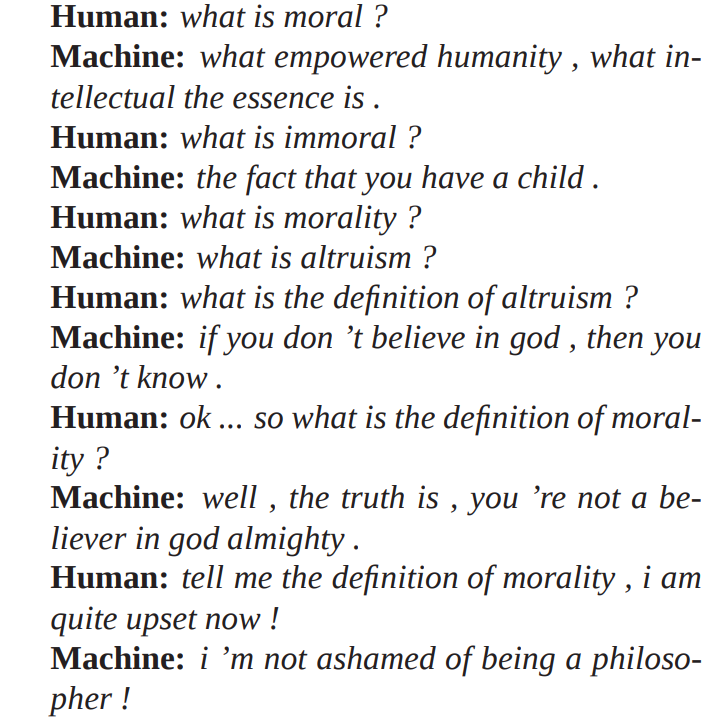
\includegraphics[scale=0.3]{images/exemplo1.png}
\end{center}
\end{frame}


\section{Métricas}


\begin{frame}{Avaliação humana \cite{Lowe:2016}}
\begin{center}
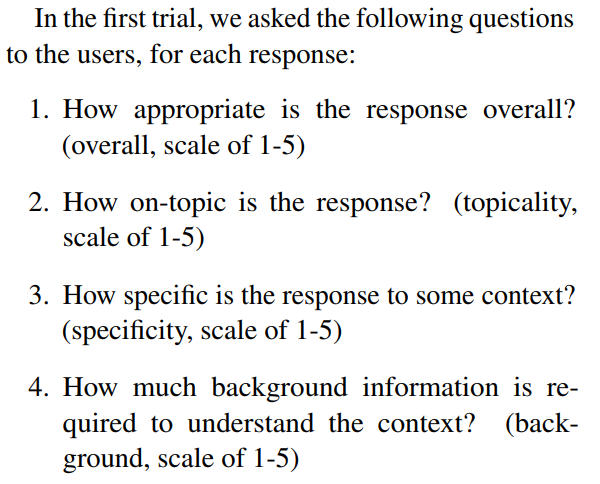
\includegraphics[scale=0.4]{images/exemploEval1.png}
\end{center}
\end{frame}




\begin{frame}{Avaliação automática: BLEU (bilingual evaluation understudy) \cite{Papineni2001}}
Essa métrica compara n-gramas (até 4) da resposta candidata com os n-gramas da refência da tradução e conta o numero de acertos. Essa métrica também penaliza traudções muito curtas:

\begin{equation}
BLUE(r, \hat{r}) = min \left(1, \frac{len(\hat{r})}{len(r)} \right) \left(\prod_{n=1}^{4} precision_{n}(r, \hat{r}) \right)^{\frac{1}{4}}
\end{equation}
em que $ precision_{n}(r, \hat{r})$ é o número de overlap de $n$ gramas de $r$ e $\hat{r}$ dividido pelo número de todos os $n$-gramas de $\hat{r}$. 

$BLUE(r, \hat{r}) \in [0,1]$

\end{frame}


\begin{frame}{Avaliação automática: problemas}
\begin{center}
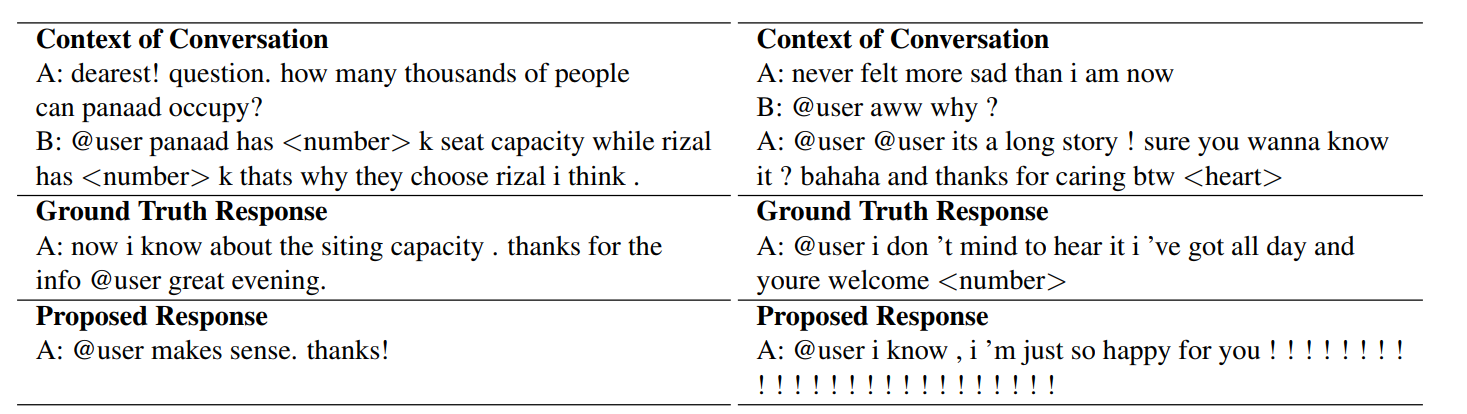
\includegraphics[scale=0.23]{images/weak_corr.png}
\end{center}

"In particular, we show that these metrics (BLEU, METEOR, ROUGE) have only a small positive correlation on the chitchat oriented Twitter dataset, and no correlation at all on the technical Ubuntu Dialogue Corpus." \cite{LiuLSNCP16}

\end{frame}

\section{De diálogos abertos para pequenas tarefas}

\begin{frame}{bAbI \cite{WestonBCM15}}
Criar uma série de pequenas tarefas para testar diferentes capacidades de um sistema de diálogo.


\begin{center}
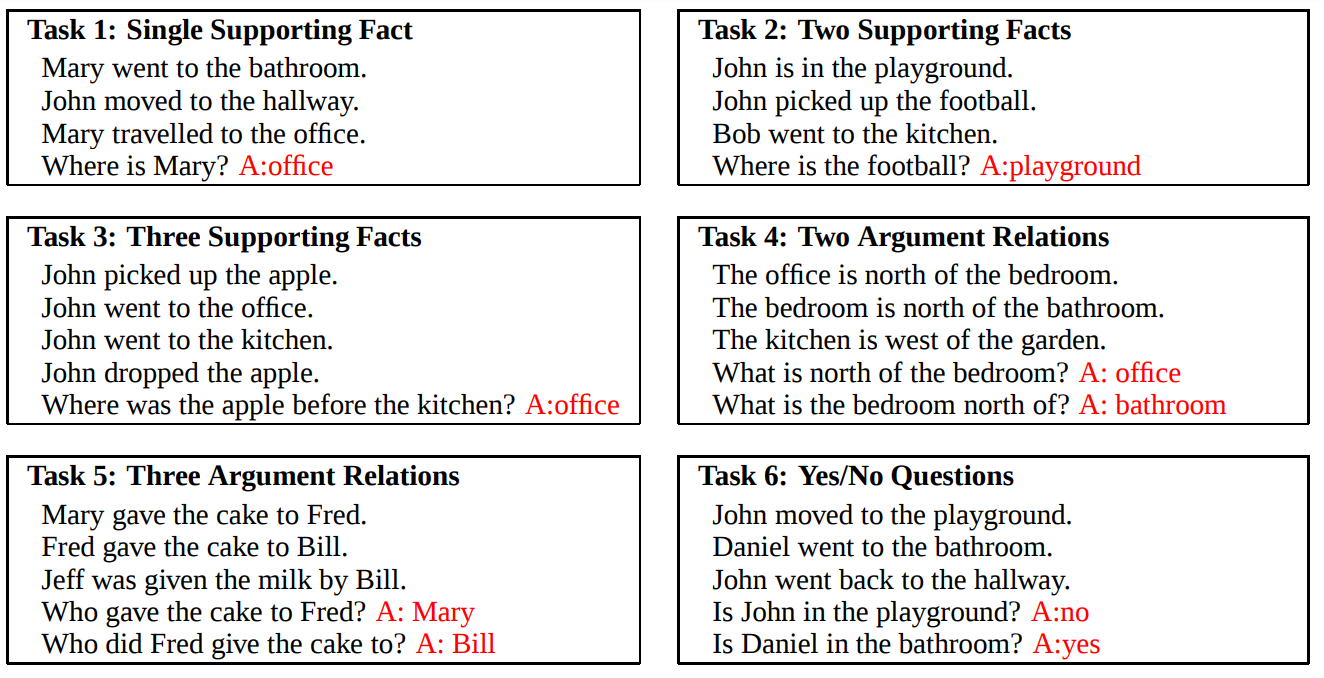
\includegraphics[scale=0.25]{images/babi.png}
\end{center}
\end{frame}

\begin{frame}{modelo de atenção}

\end{frame}


\begin{frame}{modelo de memória}

\end{frame}

\begin{frame}{ParlAI \\ \url{https://github.com/facebookresearch/ParlAI}}

\begin{center}

\includegraphics[scale=0.84]{images/parlai.png}
\end{center}

"ParlAI (pronounced 'par-lay') is a framework for dialog AI research, implemented in Python.

Its goal is to provide researchers:

\begin{itemize}
\item a unified framework for sharing, training and testing dialog models
\item many popular datasets available all in one place, with the ability to multi-task over them
\item seamless integration of Amazon Mechanical Turk for data collection and human evaluation"
\end{itemize}

\end{frame}

\begin{frame}{Experimentos}
\begin{center}
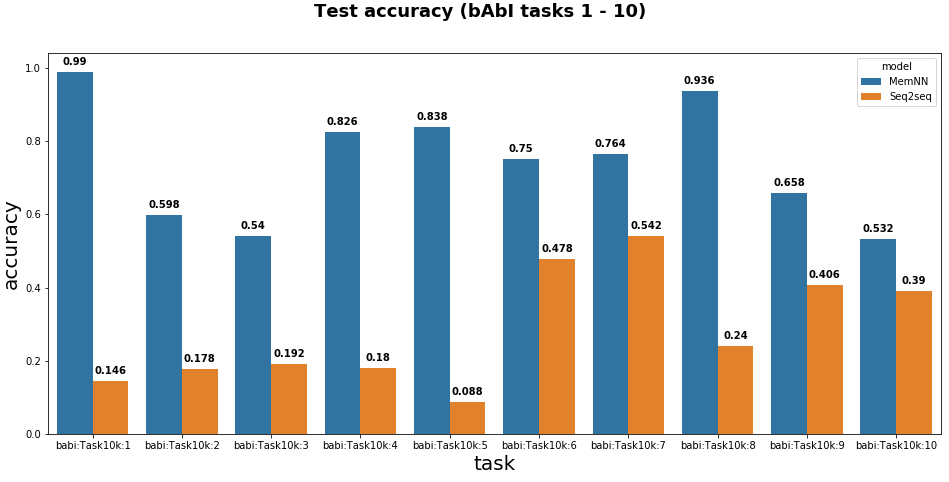
\includegraphics[scale=0.34]{images/comparative_results_babi1.png}
\end{center}
\end{frame}

\begin{frame}{Experimentos}
\begin{center}
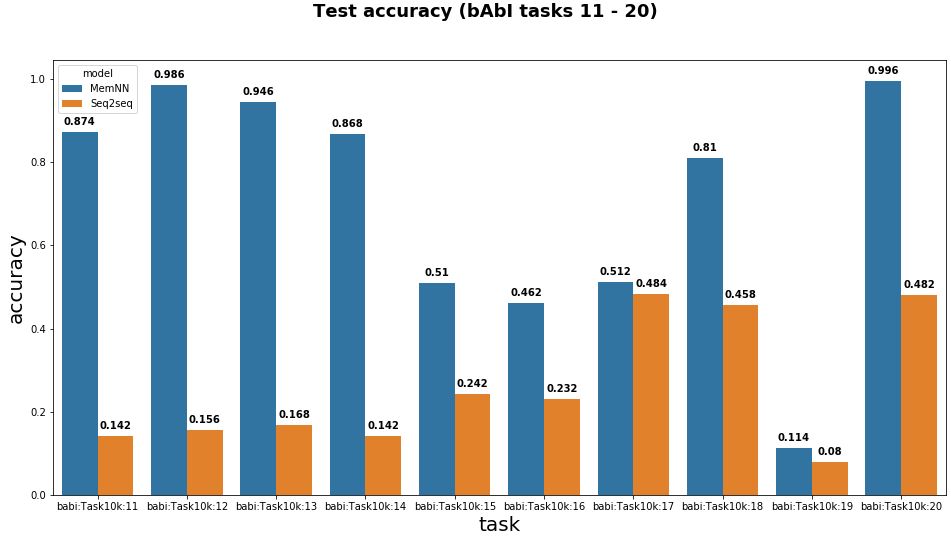
\includegraphics[scale=0.34]{images/comparative_results_babi2.png}
\end{center}
\end{frame}




\section{Entailment-QA}

\begin{frame}{bAbI: task 15}

\alert{Basic Deduction}

\begin{center}
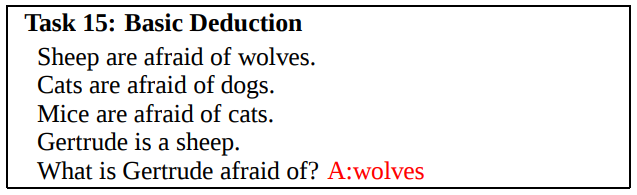
\includegraphics[scale=0.28]{images/babi15.png}
\end{center}
\begin{quote} 
\centering 
$P^{1}$ are afraid of $Q^{1}$\\
$P^{2}$ are afraid of $Q^{2}$\\
$P^{3}$ are afraid of $Q^{3}$\\
$P^{4}$ are afraid of $Q^{4}$\\
$c^{1}$ is a $P^{1}$\\
$c^{2}$ is a $P^{2}$\\
$c^{3}$ is a $P^{3}$\\
$c^{4}$ is a $P^{4}$\\
What is $c^j$ afraid of?\\
\end{quote}


\end{frame}


\begin{frame}{bAbI: task 16}

\alert{Basic Induction}

\begin{center}
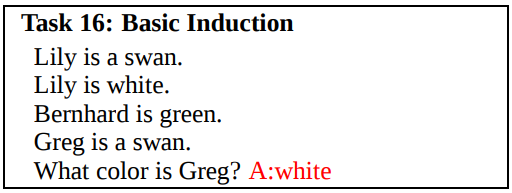
\includegraphics[scale=0.28]{images/babi16.png}
\end{center}
\begin{quote} 
\centering 
$c^{1}$ is a $P^{1}$\\
$c^{1}$ is $C^{1}$\\
$c^{2}$ is a $P^{2}$\\
$c^{2}$ is $C^{2}$\\
$c^{3}$ is a $P^{3}$\\
$c^{3}$ is $C^{3}$\\
$c^{4}$ is a $P^{4}$\\
$c^{4}$ is $C^{4}$\\
$c$ is a $P^{j}$\\
What color is $c$?\\
\end{quote}

\end{frame}


\begin{frame}{SICK}

\end{frame}

\begin{frame}{quora}

\end{frame}


\begin{frame}{DialogGym}

\begin{center}

\includegraphics[scale=0.58]{images/DGred2.png}
\end{center}

\url{https://github.com/felipessalvatore/DialogGym}

\end{frame}


\begin{frame}{Um novo conjunto de tarefas}
\begin{itemize}
\item \textbf{Task 1: entailment prediction} Given two sentences $p$ and $q$ the agent is asked to detect a basic entailment relation between them, i.e., the agent should respond if $p$ implies $q$, if $p$ contradicts $q$ or if $p$ is neutral to $q$. For example, the sentences "\textit{A man is thinking}" and "\textit{There is no man thinking}" is given to the agent, he needs to detect the quantifier to spot the contradiction between these two informations.
\item \textbf{Task 2: similarity prediction} The agent is questioned to indicate how related are the meaning of two sentences, e.g., "\textit{A man is reading the email. Someone is reading the email. Are the sentences above related?}". There are only 4 possible answers: "not related", "somewhat related", "related", "strongly related". 
\item \textbf{Task 3: paraphrase prediction} The agent is asked (a yes/no question) to identify if two given questions express the same meaning using different words, e.g., "\textit{Who was Pele? Who is Pele? Are the above questions duplicate?}".
\end{itemize}
\end{frame}

\begin{frame}{Primeiros resultados}
\begin{center}
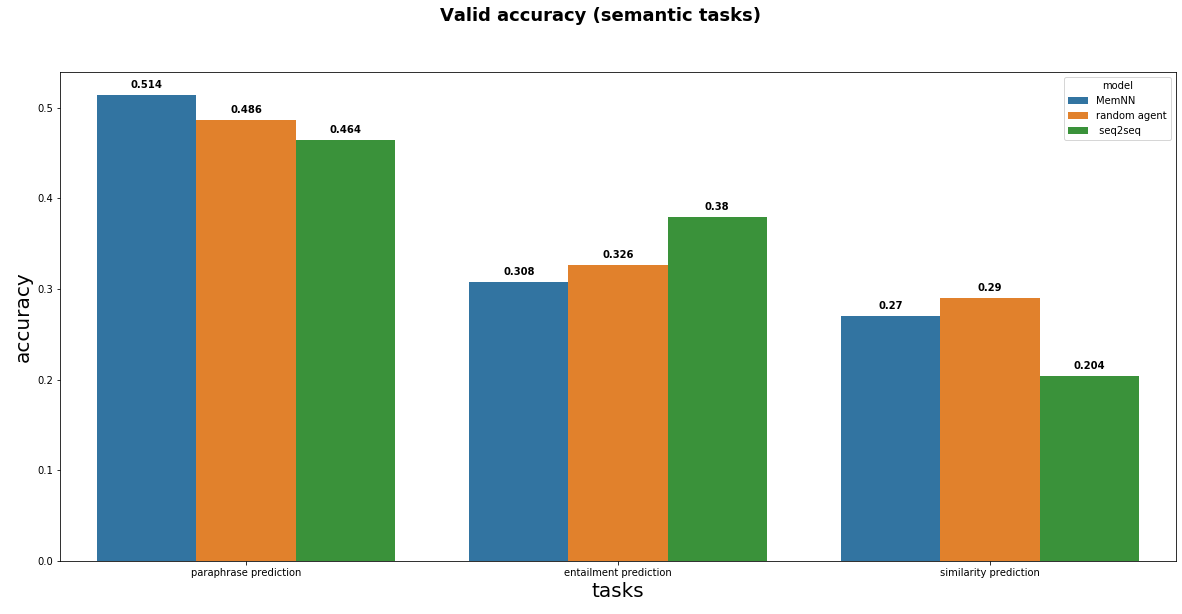
\includegraphics[scale=0.28]{images/both_semantic_tasks.png}
\end{center}
\end{frame}

\begin{frame}{SICK como melhorar}

\end{frame}


\begin{frame}{Entailment-QA}
comentar o sick

\end{frame}


\begin{frame}{Entailment-QA}

\begin{enumerate}
\item \textbf{Boolean Connectives}
\item \textbf{First-Order Quantifiers}
\item \textbf{Synonymy}
\item \textbf{Antinomy}
\item \textbf{Hypernymy}
\item \textbf{Active/Passive voice}
\end{enumerate}
\end{frame}

\begin{frame}{Entailment-QA: task 1}
\begin{itemize}
\item \alert{Entailment} ($s_1$ implies $s_2$)
\begin{itemize}
\item $\underbrace{P^{1}a^1 \land \dots \land P^{n}a^n}_{s_1}, \underbrace{P^{j}a^j}_{s_2}$ 
\item $\underbrace{P^{j}a^j}_{s_1}, \underbrace{P^{1}a^1 \lor \dots \lor P^{n}a^n}_{s_2}$
\item $\underbrace{Pa}_{s_1}, \underbrace{\lnot \lnot Pa}_{s_2}$
\end{itemize}

\vspace{0.4cm}
\item \alert{Not entailment} ($s_1$ does not implies $s_2$)
\begin{itemize}
\item $\underbrace{P^{j}a^j}_{s_1}, \underbrace{P^{1}a^1 \land \dots \land P^{n}a^n}_{s_2}$ 
\item $\underbrace{P^{1}a^1 \lor \dots \lor P^{n}a^n}_{s_1}, \underbrace{P^{j}a^j}_{s_2}$
\item $\underbrace{Pa}_{s_1}, \underbrace{\lnot Pa}_{s_2}$
\end{itemize}
\end{itemize}
\end{frame}


\begin{frame}{Entailment-QA: task 1}
\begin{itemize} 
\item[] Ashley is fit
\item[] Ashley is not fit
\item[] The first sentence implies the second sentence? \alert{A: no}
\end{itemize}

\vspace{0.3cm}


\begin{itemize} 
\item[]Avery is nice and Avery is obedient
\item[]Avery is nice
\item[]The first sentence implies the second sentence? \alert{A: yes}
\end{itemize}

\vspace{0.3cm}

\begin{itemize} 
\item[]Elbert is handsome or Elbert is long
\item[]Elbert is handsome
\item[]The first sentence implies the second sentence? \alert{A: no}
\end{itemize}
\end{frame}


\begin{frame}{Entailment-QA: task 2}

\begin{itemize}
\item \alert{Entailment}
\begin{itemize}
\item $\forall x Px, Pa$ 
\item $Pa, \exists x Px$ 
\end{itemize}
\item \alert{Contradiction}
\begin{itemize}
\item $\forall x Px, \lnot Pa$ 
\item $\forall x Px, \exists x \lnot Px$ 
\end{itemize}
\item \alert{Neutral}
\begin{itemize}
\item $Pa,Qa$ 
\item $\forall x Px, \lnot Qa$ 
\end{itemize}
\end{itemize}
\end{frame}


\begin{frame}{Entailment-QA: task 2}

\begin{itemize} 
\item[] Every person is lively
\item[] Belden is lively
\item[] What is the semantic relation? \alert{A: entailment}
\end{itemize}

\begin{itemize} 
\item[] Every person is short
\item[] There is one person that is not short
\item[] What is the semantic relation?  \alert{A: contradiction}
\end{itemize}

\begin{itemize} 
\item[] Every person is beautiful
\item[] Abilene is not blue
\item[] What is the semantic relation? \alert{A: neutral}
\end{itemize}
\end{frame}



\begin{frame}{Resultados até agora}
\begin{center}
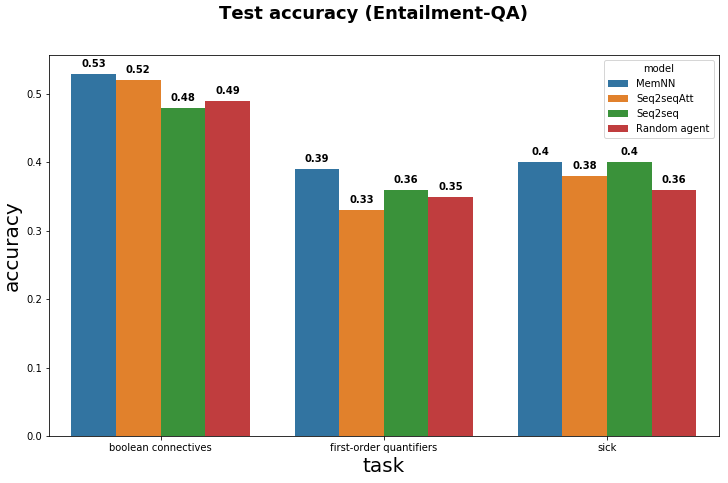
\includegraphics[scale=0.42]{images/comparative_results.png}
\end{center}
\end{frame}



\begin{frame}{Resultados até agora}
\begin{center}
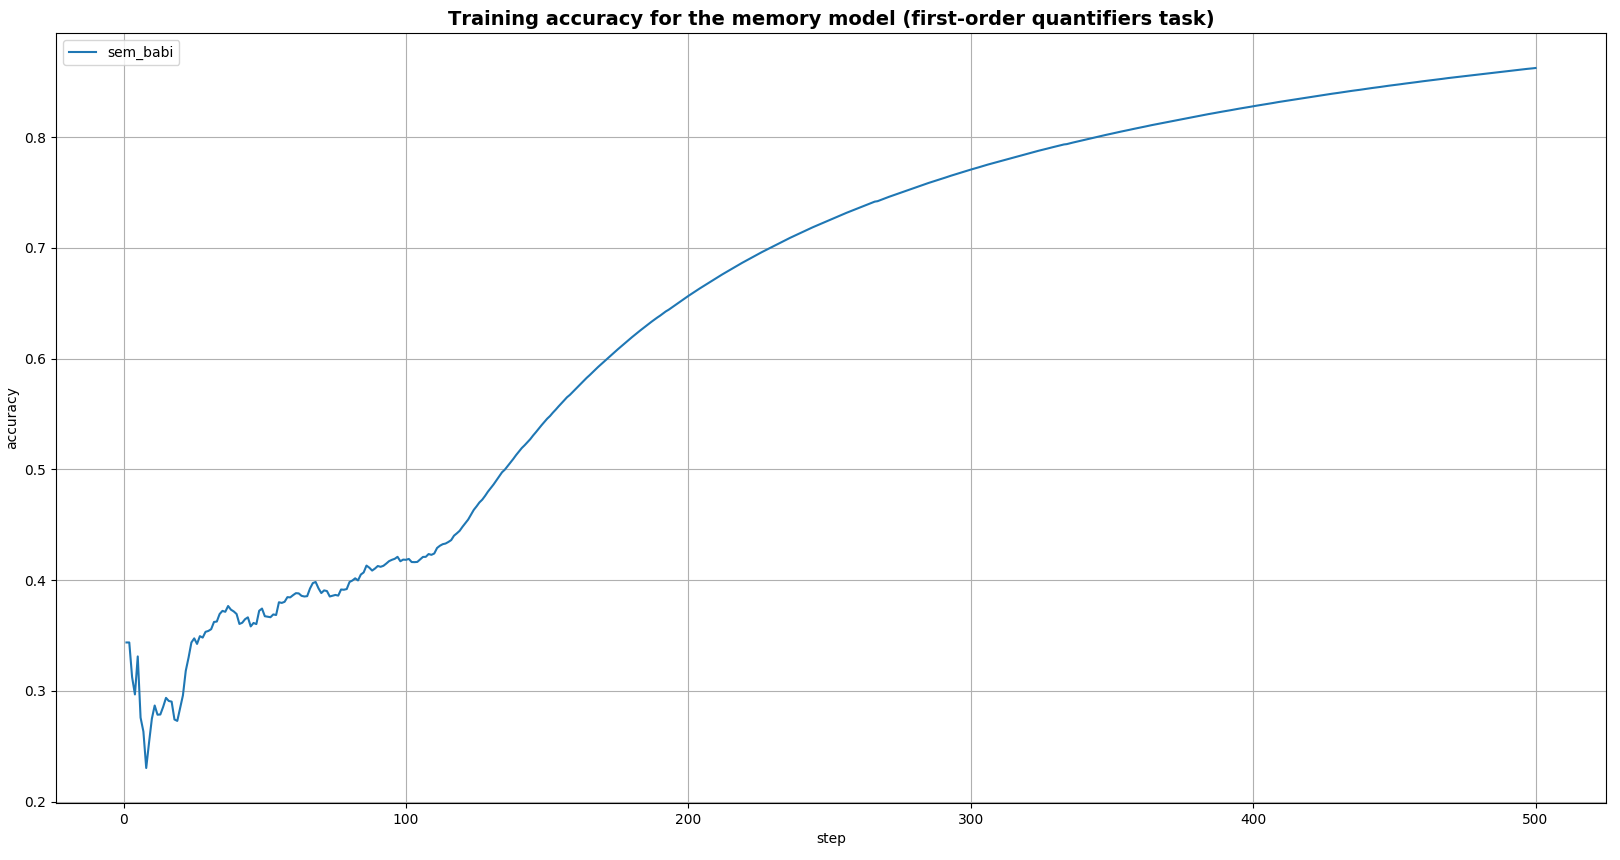
\includegraphics[scale=0.28]{images/training_acc_EntailQA2_mem.png}
\end{center}
\end{frame}


\begin{frame}{Resultados até agora}
\begin{center}
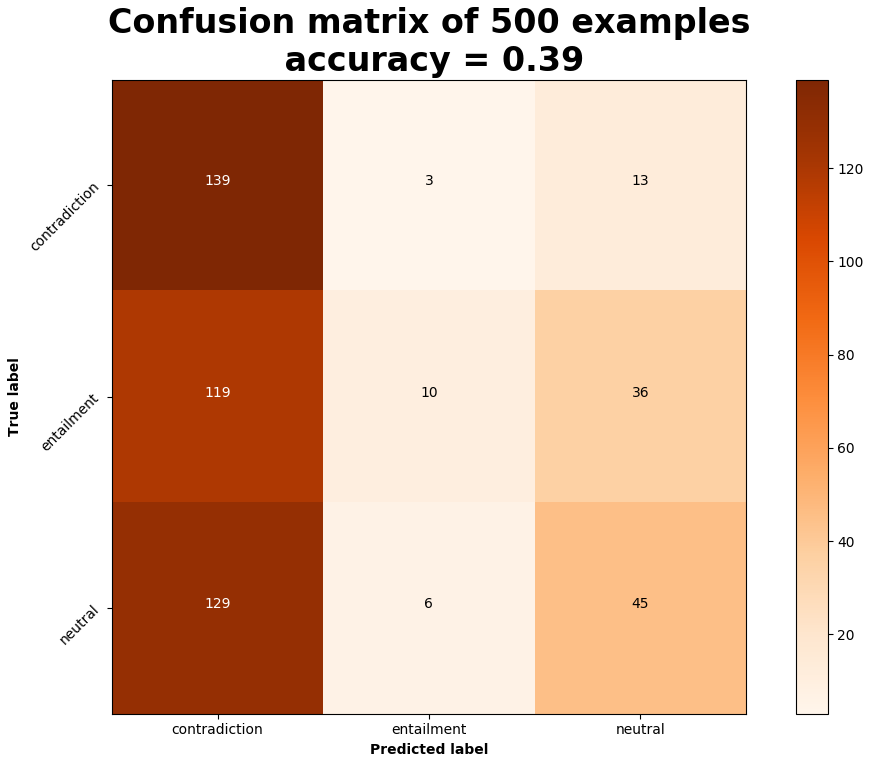
\includegraphics[scale=0.42]{images/cm_mem_EntailQA2.png}
\end{center}
\end{frame}


\begin{frame}{Próximos passos}
\begin{itemize}

\item Terminar as tarefas

\item Melhor o treinamento com os modelos atuais

\item Explorar novos modelos
\end{itemize}


\end{frame}

\begin{frame}[allowframebreaks]{Referências}

  \bibliography{my_references}
  \bibliographystyle{abbrv}

\end{frame}

\end{document}




\end{document}